\addsection{Resources}{\images/estates.png}
There are three types of resources in the game: gold, building materials, and valuables.
Resources are spent during the game to expand your town, to recruit units, and to purchase spells.
You can gain resources from settlements and mines that you have \hyperlink{Categories}{flagged}, but also by using artifacts and rolling resource dice \includesvg[height=10px]{\svgs/resource_die.svg}.
Whenever a player's resource production is increased or decreased, move that resource's cube on its production track the appropriate number of spaces.\par
\begin{figure}[h]
  \centering
  \minipage[b]{0.32\textwidth}
    \centering
    
\includegraphics[scale=0.2]{\images/gold.png}
    \caption{{\textit{\textbf{\textcolor{purple}{Gold}}}}}
  \endminipage
  \minipage[b]{0.32\textwidth}
    \centering
    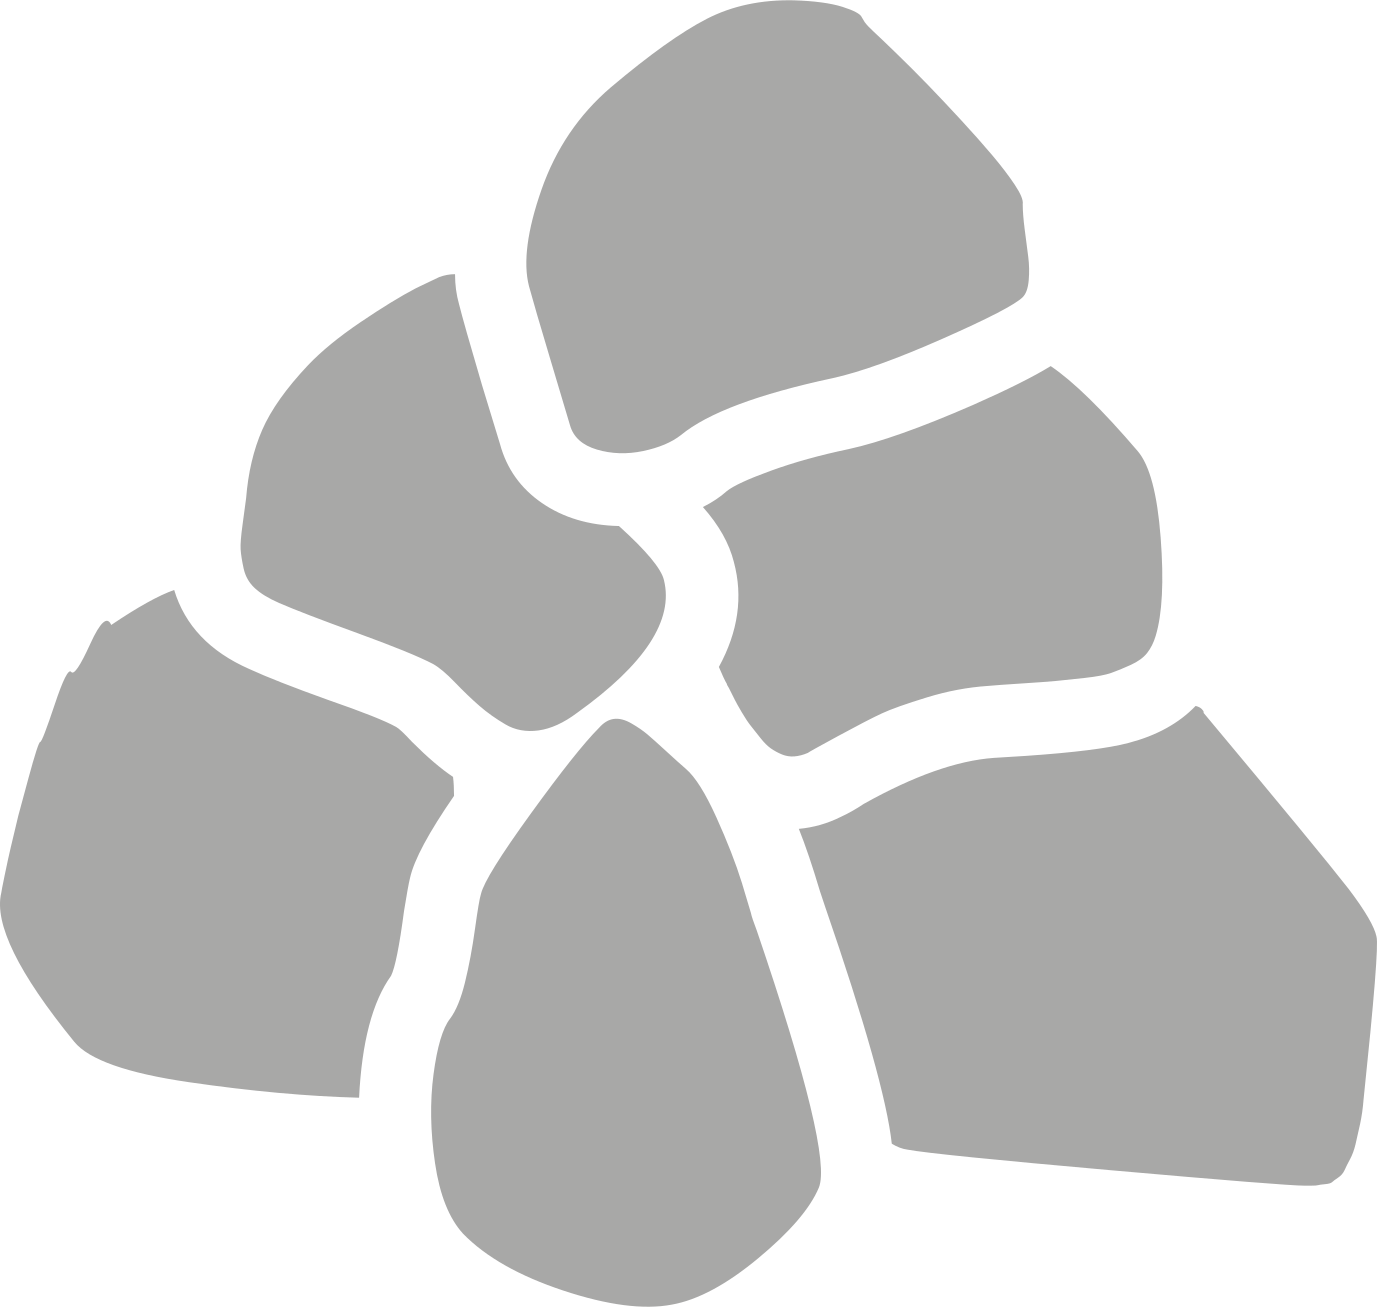
\includegraphics[scale=0.2]{\images/building_materials.png}
    \caption{{\textit{\textbf{{\textcolor{purple}{Building Materials}}}}}}
  \endminipage
  \minipage[b]{0.32\textwidth}
    \centering
    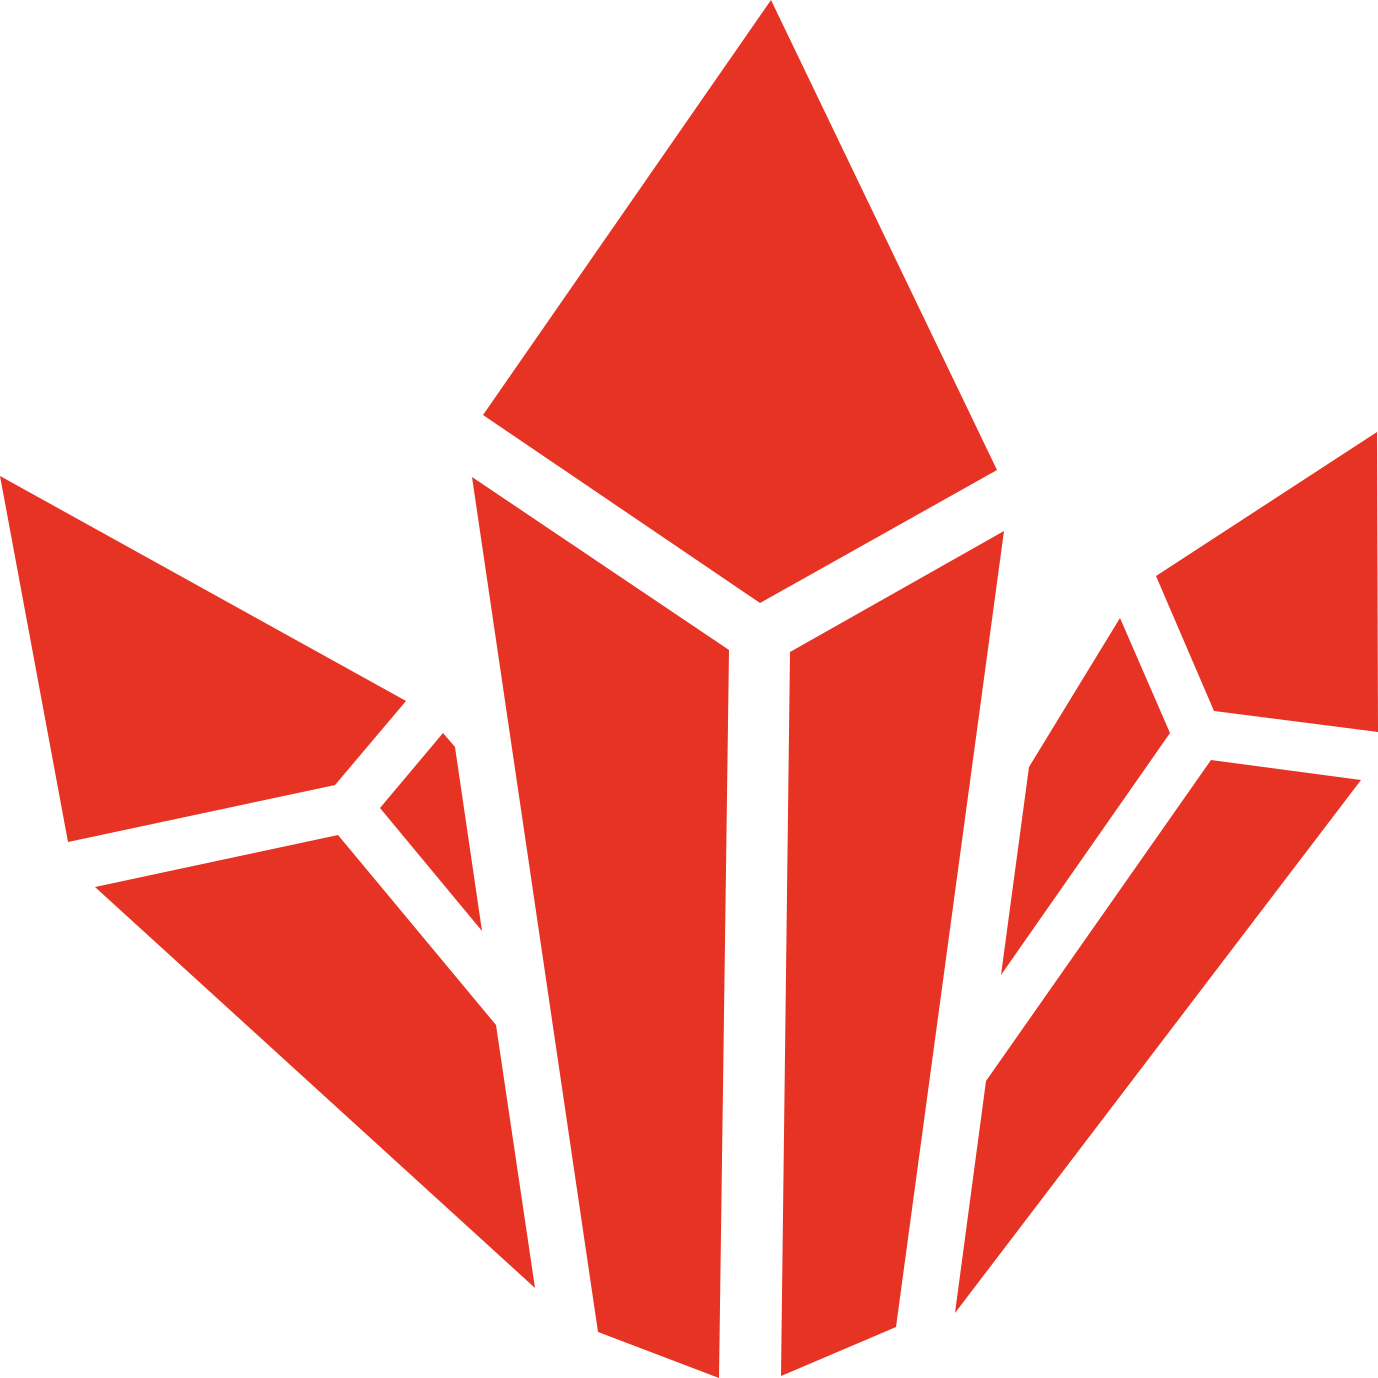
\includegraphics[scale=0.2]{\images/valuables.png}
    \caption{{\textit{\textbf{{\textcolor{purple}{Valuables}}}}}}
  \endminipage
\end{figure}
Players start each scenario with the number of resources indicated in that scenario’s set up.
Resources can also be \hyperlink{Trading}{traded}.
There's no limit to the amount of resources you can have.
% TODO Fill this new resource page with resource dice results etc.
